\documentclass[tikz,border=2pt]{standalone}
\usepackage{tikz}
\usepackage{lmodern}
\usetikzlibrary{calc,decorations.pathreplacing}

% Visual conventions follow the existing MRNC TikZ pictures: ordinary
% components use TikZ's normal 0.4pt stroke, with compact TeX labels.
\tikzset{
  nu fibre/.style={
    x=0.78cm,
    y=0.78cm,
    line width=0.4pt,
    line cap=round,
    line join=round
  },
  nu label/.style={
    font=\scriptsize,
    inner sep=1pt
  },
  nu annotation/.style={
    font=\scriptsize,
    inner sep=1pt
  },
  nu dots/.style={
    font=\small,
    inner sep=0pt
  }
}

\begin{document}

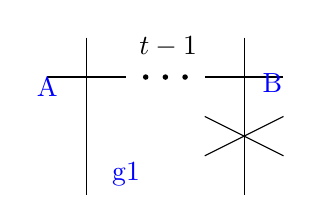
\begin{tikzpicture}[scale=0.5]
 % chain 
  \coordinate (C) at (-1.50, 3.00);
  \coordinate (D) at (-0.50, 3.00);
  \coordinate (A) at (-1.00, 3.00);
  \coordinate (B) at (-0.93, 3.26);
\node[above] at (B) {$t-1$};
  \fill[black] (C) circle (2pt);
  \fill[black] (D) circle (2pt);
  \fill[black] (A) circle (2pt);
 
 %I_0
 \coordinate (I0A) at (-4.00, 3.00);
  \coordinate (I0B) at (-2.00, 3.00);
  \coordinate (I0C) at (-3.00, 4.00);
  \coordinate (I0D) at (-3.00, 0.00);
  \coordinate (I0A_1) at (-4.00, 2.25);
  \coordinate (I0E) at (-2.00, 0.00);
 \draw (I0A) -- (I0B);
  \draw (I0C) -- (I0D);
  \node[above, text=blue] at (I0A_1) {A};
  \node[above, text=blue] at (I0E) {g1};

%IV 

  \coordinate (IVrC) at (0.00, 3.00);
  \coordinate (IVrD) at (2.00, 3.00);
  \coordinate (IVrE) at (1.00, 4.00);
  \coordinate (IVrF) at (1.00, 0.00);
  \coordinate (IVrG) at (0.00, 2.00);
  \coordinate (IVrL) at (2.00, 1.00);
  \coordinate (IVrI) at (0.00, 1.00);
  \coordinate (IVrM) at (2.00, 2.00);
  \coordinate (IVrD_1) at (1.72, 2.35);

  

  \draw (IVrC) -- (IVrD);
  \draw (IVrE) -- (IVrF);
  \draw (IVrG) -- (IVrL);
  \draw (IVrI) -- (IVrM);
  \node[above, text=blue] at (IVrD_1) {B};
\end{tikzpicture}

\end[document}
